\section{The SkelCL Programming Model}
\label{section:skelcl-programming-model}
\SkelCL (Skeleton Computing Language) is a high-level programming model targeting multi-\GPU system.
It is developed as an extension of the standard \OpenCL programming model~\cite{OpenCL}.

\SkelCL adds three main high-level features to \OpenCL which we identified as desirable in~\autoref{section:requirements}:

\begin{itemize}
  \item \emph{parallel container data types} for unified memory management between \CPU and (multiple) \GPUs;
  \item \emph{recurring patterns of parallelism} (\aka \emph{algorithmic skeletons}) for easily expressing parallel computation patterns;
  \item \emph{data distribution} and \emph{redistribution} mechanisms for transparent data transfers in multi-\GPU systems.
\end{itemize}

\noindent
\SkelCL inherits all advantageous properties of \OpenCL, including its portability across different heterogeneous parallel systems.
\SkelCL is designed to be fully compatible with \OpenCL: arbitrary parts of a \SkelCL code can be written or rewritten in \OpenCL, without influencing program's correctness.

In the remainder of this section we discuss the design of the \SkelCL programming model in more detail.
Its implementation as a \Cpp library will be discussed in the next section.

% ============================================================================ %
\subsection{Parallel Container Data Types}
\label{section:skelcl-programming-model:container}
\SkelCL offers the application developer two container classes -- vector and matrix -- which are transparently accessible by both, \CPU and \GPUs (or using \OpenCL's terminology, host and devices).
The \emph{vector} abstracts a one-dimensional contiguous memory area while the \emph{matrix} provides an interface to a two-dimensional memory area.

When a container is created on the host, memory is allocated on the devices automatically;
when a container on the host is deleted, the memory allocated on the devices is freed automatically.

The main advantage of the container data types in \SkelCL as compared with \OpenCL is that the necessary data transfers between the host and devices are performed automatically and implicitly.
Before performing a computation on container types, the \SkelCL system ensures that all input containers' data is available on all participating devices.
This may result in implicit data transfers from the host to device memory, which in \OpenCL would require explicit programming, as we saw in~\autoref{section:opencl-example}.
Similarly, before any data is accessed on the host, the implementation of \SkelCL implicitly ensures that this data on the host is up-to-date by performing necessary data transfers automatically.
Thus, the container classes shield the programmer from low-level operations like memory allocation (on the devices) and data transfers between host and device.

Developing applications on two-dimensional data for modern parallel architectures is cumbersome and challenging, since efficient memory handling is essential for achieving good performance.
In case of \GPUs, exploiting the memory hierarchy by using the fast but small on-chip memory is key for high performance.
Therefore, in addition to the vector as a one-dimensional abstract data structure, \SkelCL offers a specific abstract data type for handling two-dimensional data, the matrix.

% The implementations of the algorithmic skeletons included in \SkelCL differentiate for their input container between vector and matrix, thus, offering optimized implementations for each case.


\subsection{Algorithmic Skeletons}
\label{section:skelcl-programming-model:skeletons}
In original \OpenCL, computations are expressed as compute \emph{kernels} which are executed in a parallel manner on an \OpenCL device, \eg, a \GPU.
As seen earlier the application developer must explicitly specify the parallelism by indicating how many instances of a kernel (called \emph{work items}) should be launched in parallel.
Communications between work items are limited and have to be implemented carefully to avoid race conditions and deadlocks.
In addition, kernels take unsafe pointers to device memory as input and contain program code for reading/writing single data items from/to it.
These pointers have to be used carefully, because no boundary checks are performed by \OpenCL.

To shield the application developer from these low-level programming issues, \SkelCL extends \OpenCL by introducing high-level programming patterns, called \emph{algorithmic skeletons}~\cite{Cole1991}.
Formally, a skeleton is a higher-order function that executes one or more user-defined (so-called \emph{customizing}) functions in a pre-defined parallel manner, thus hiding the details of parallelism and communication from the user~\cite{GorlatchCo2011}.

\SkelCL provides four basic data-parallel skeletons: \map, \zip, \reduce, and \scan,
as well as two more advanced skeletons targeting specific application domains: \stencil and \allpairs.
In this section we will look at the basic skeletons, the advanced skeletons will be discussed in~\autoref{section:skelcl-programming-model:specialSkeletons}.
The four basic skeletons have been selected, because they have been proven to be useful for a broad range of applications.
Moreover, these skeletons can be efficiently implemented on \GPUs as their computation patterns match the data-parallel \SIMD (Singe Instruction, Multiple Data) execution model implemented by \GPUs.


\paragraph{The \map skeleton}
The \map skeleton is a well-known basic algorithmic skeleton, applying the customizing function to each element of a container in parallel.
This skeleton originates from the functional world, where the \code{map} function is recognized as an important primitive for writing high-level code.
In many programming languages an equivalent sequential function exists, either known under the same name, like in Haskell or Python, or by other names, like \code{transform} in \Cpp.

In \SkelCL the \map skeleton can operate on vectors as well as matrices.
We start by formally defining the skeleton on vectors:
\begin{definition}
  \label{definition:map}
  Let $\vec{x}$ be a vector of size $n$ with elements $x_i$ where $0 < i \leq n$.
  Let $f$ be a unary customizing function defined on elements.
  The algorithmic skeleton \map is then defined as follows:
  \begin{equation*}
    map \big(\ f,\ [x_1, x_2, \dots, x_n]\ \big) \eqdef [f(x_1), f(x_2), \dots, f(x_n)]
  \end{equation*}
\end{definition}
\noindent
The definition for matrices is similar:
\begin{definition}
  \label{definition:map:matrix}
  Let $M$ be an $n\times m$ matrix with elements $M_{i,j}$ where $0 < i \leq n$ and $0 < j \leq m$.
  Let $f$ be a unary customizing function.
  The algorithmic skeleton \map is defined as follows:
  \begin{equation*}
    map\big(\ f,\ \DottedMatrix{M_{0,0}}{M_{0,m}}{M_{n,0}}{M_{n,m}} \big)
      \eqdef \DottedMatrix{f(M_{0,0})}{f(M_{0,m})}{f(M_{n,0})}{f(M_{n,m})}
  \end{equation*}
\end{definition}
\noindent
The output container of the \map skeleton, either vector or matrix, can be computed in parallel, because the computation of each single element is independent of each other.

A simple possible application of the \map skeleton is negating all the values in a vector:
\begin{align*}
  neg(\vec{x}) &= map(\ -, \vec{x}\ )
\end{align*}


\paragraph{The \zip skeleton}
The \zip skeleton operates on two containers and combines them into one.
As the \map skeleton it is defined for vectors and matrices as well.
\begin{definition}
  \label{definition:zip}
  Let $\vec{x}$ and $\vec{y}$ be vectors of size $n$ with elements $x_i$ and $y_i$ where $0 < i \leq n$.
  Let $\oplus$ be a binary customizing operator.
  The algorithmic skeleton \zip is defined as follows:
  \begin{equation*}
    \begin{split}
    zip \big(\ \oplus,\ [x_1, x_2, \dots, x_n],\ [y_1, y_2, \dots, y_n]\ \big)\\
      \eqdef [x_1 \oplus y_1, x_2 \oplus y_2, \dots, x_n \oplus y_n]
    \end{split}
  \end{equation*}
\end{definition}
\noindent
Again the definition for matrices is similar:
\begin{definition}
  \label{definition:zip:matrix}
  Let $A$ and $B$ be $n\times m$ matrices with elements $A_{i,j}$ and $B_{i,j}$ where $0 < i \leq n$ and $0 < j \leq m$.
  Let $\oplus$ be a binary customizing operator.
  The algorithmic skeleton \zip is defined as follows:
  \begin{equation*}
    \begin{split}
    zip\big( f,\ {\DottedMatrix{A_{0,0}}{A_{0,m}}{A_{n,0}}{A_{n,m}}},\
                 {\DottedMatrix{B_{0,0}}{B_{0,m}}{B_{n,0}}{B_{n,m}}}\big) \\
      \eqdef \DottedMatrix{A_{0,0} \oplus B_{0,0}}{A_{0,m} \oplus B_{0,m}}{A_{n,0} \oplus B_{n,0}}{A_{n,m} \oplus B_{n,m}}
    \end{split}
  \end{equation*}
\end{definition}
\noindent
This definitions require the two input containers to be of exactly the same size.
The \zip skeleton is parallelizeable in the same manner as \map, as each element of the output container can be computed in parallel.

A possible application of the \zip skeleton is performing pairwise addition of two vectors:
\begin{align*}
  add(\vec{x},\ \vec{y}) = zip(\ +, \vec{x},\ \vec{y}\ )
\end{align*}


\paragraph{The \reduce skeleton}
The \reduce skeleton computes a single value from a vector by successively applying the binary customizing function.
In \SkelCL the \reduce skeleton is only defined on vectors:
\begin{definition}
  \label{definition:reduce}
  Let $\vec{x}$ be a vector of size $n$ with elements $x_i$ where $0 < i \leq n$.
  Let $\oplus$ be an associative and commutative, binary customizing operator with the corresponding identity element $id$.
  The algorithmic skeleton \reduce is defined as follows:
  \begin{equation*}
    reduce \big(\ \oplus,\ id,\ [x_1, x_2, \dots, x_n]\ \big)
      \eqdef x_1 \oplus x_2 \oplus \dots \oplus x_n
  \end{equation*}
\end{definition}
\noindent
Requiring the operator to be associative and commutative enables efficient parallel implementations.
The identity element $id$ can be used by the implementation, \eg, to initialize intermediate buffers.

A possible application of the \reduce skeleton is to finding the maximum value of a vector:
\begin{align*}
  maxValue(\vec{x}) &= reduce(\ max,\ 0,\ \vec{x}\ )\\
  \text{where:} \qquad max(a, b) &=
    \left\{
      \begin{array}{l l}
      a & \text{if } a \geq b\\
      b & \text{if } a < b
      \end{array}
    \right.
\end{align*}


\paragraph{The \scan skeleton}
The \scan skeleton (\aka prefix-sum) yields an output vector with each element obtained by applying the customizing function to the elements of the input vector up to the current element's index.
In \SkelCL, the \scan skeleton is only defined on vectors:
\begin{definition}
  \label{definition:scan}
  Let $\vec{x}$ be a vector of size $n$ with elements $x_i$ where $0 < i \leq n$.
  Let $\oplus$ be an associative binary customizing operator with the corresponding identity element $id$.
  The algorithmic skeleton \scan is defined as follows:
  \begin{equation*}
    \begin{split}
    scan \big(&\ \oplus,\ id,\ [x_1, x_2, \dots, x_n]\ \big) \\
      &\eqdef [id, x_1 \oplus x_2,\ \dots,x_1 \oplus x_2 \oplus \cdots \oplus x_n]
    \end{split}
  \end{equation*}
\end{definition}
\noindent
Even though the \scan pattern seems inherently sequential, because each individual result contains the results of its predecessor, efficient parallel implementations do exist for this problem.
Blelloch~\cite{Blelloch1991} studies this parallel pattern in great detail and efficient implementations for \GPUs exist~\cite{HarrisSeOw2007} following his algorithmic ideas.

A possible application of the \scan skeleton is the computation of the prefix sum which can be used as part of the counting sort algorithm~\cite{Knuth1998} or for solving the list ranking problem~\cite{ColeVi1989}.
\begin{align*}
  prefixSum(\vec{x}) = scan(\ +,\ 0,\ \vec{x}\ )
\end{align*}

\paragraph{Parallel Programming with Algorithmic Skeletons}
In \SkelCL, rather than writing low-level kernels, the application developer customizes suitable skeletons by providing application-specific functions which are often much simpler than kernels as they specify an operation on basic data items rather than containers.
Skeletons can be executed on both single- and multi-device systems.
In case of a multi-device system, the calculation specified by a skeleton is performed automatically on all devices available in the system.

Skeletons can be customized and composed to express more complex algorithms.
To demonstrate how to express computations with algorithmic skeletons let us consider three simple linear algebra applications:
scaling a vector with a constant, computing the sum of absolute values of a vector, and computing the dot product (\aka inner product) of two vectors.
These three applications are all part of the well-known \emph{Basic Linear Algebra Subprograms (\BLAS)}~\cite{Dongarra2002,Dongarra2002a} library.

For scaling a vector with a constant $\alpha$ we use the \map skeleton:
\begin{align*}
  scal(\vec{x}) &= map(\ f_{\alpha}, \vec{x}\ )\\
  \text{where:} \qquad f_{\alpha}(x_i) &= \alpha \cdot x_i
\end{align*}

\noindent
For computing the sum of absolute values we compose a \map and \reduce skeleton.
We use the $\circ$ to denote the sequential composition of two functions, \ie\ $(f \circ g)(x) = f(g(x))$.
\begin{align*}
  asum(\vec{x}) &= reduce(\ +,\ 0\ ) \circ map(\ abs, \vec{x}\ )\\
  \text{where:} \qquad abs(a) &=
    \left\{
      \begin{array}{r l}
      a & \text{if } a \geq 0\\
      -a & \text{if } a < 0
      \end{array}
    \right.
\end{align*}

\noindent
To compute the dot product of two vectors we compose a \zip skeleton customized with multiplication and a \reduce skeleton customized with addition:
\begin{align*}
  dot(\vec{x}, \vec{y}) &= reduce(\ +,\ 0\ ) \circ zip(\ \times, \vec{x}, \vec{y}\ )
\end{align*}

\noindent
Algorithmic skeletons are not limited to linear algebra applications, but can be used to implement a boarded range of application types as we will discuss in \autoref{chapter:skelcl-evaluation}.
Among others, we will see an implementation using algorithmic skeletons of the real-world medial imaging application example discussed at the beginning of this chapter.


% ============================================================================ %
\subsection{Data distribution and redistribution}
\label{section:skelcl-programming-model:distribution}

For multi-device systems, \SkelCL's parallel container data types (vector and matrix) abstract from the separate memory areas on multiple \OpenCL devices, \ie, container's data is accessible by each device.
Each device may access different parts of a container or may even not access it at all.
For example, when implementing work-sharing on multiple \GPUs, the \GPUs will access disjoint parts of input data, such that copying only a part of the vector to a \GPU would be more efficient than copying the whole data to each \GPU.

To simplify the partitioning of a container on multiple devices, \SkelCL introduces the concept of \emph{distributions}.
A distribution describes how the container's data is distributed among the available devices.
It allows the application developer to abstract from the challenges of managing memory ranges which are shared or partitioned across multiple devices: the programmer can think of a distributed container as of a self-contained entity.



\begin{figure}[tb]
  \centering
  \begin{subfigure}{.3\textwidth}
    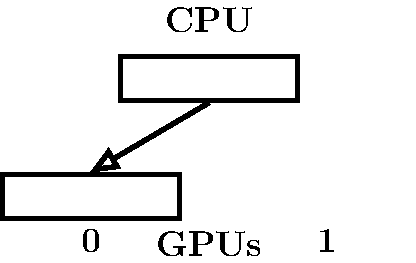
\includegraphics[width=\textwidth]{PaCT/singleDistribution_vector}
    \caption{\emph{single}}
    \label{fig:distributions:single}
  \end{subfigure}
  \hfill
  \begin{subfigure}{.3\textwidth}
    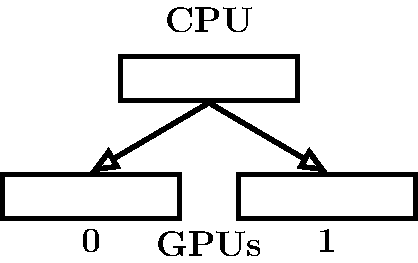
\includegraphics[width=\textwidth]{PaCT/copyDistribution_vector}
    \caption{\emph{copy}}
    \label{fig:distributions:copy}
  \end{subfigure}
  \hfill
  \begin{subfigure}{.3\textwidth}
    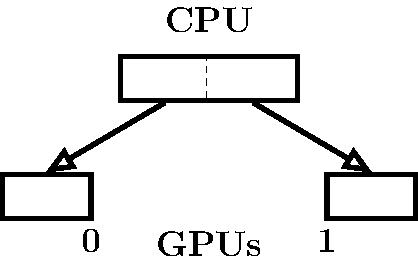
\includegraphics[width=\textwidth]{PaCT/blockDistribution_vector}
    \caption{\emph{block}}
    \label{fig:distributions:block}
  \end{subfigure}
  \caption{Distributions of a vector in SkelCL.}
  \label{fig:distributions}
  \bigskip
\end{figure}

\begin{figure}[tbp]
  \centering
  \begin{subfigure}{.22\textwidth}
    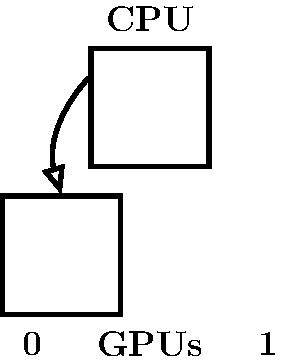
\includegraphics[width=\textwidth]{PaCT/singleDistribution_matrix}
    \caption{\emph{single}}
    \label{fig:distributions_matrix:single}
  \end{subfigure}
  \hfill
  \begin{subfigure}{.22\textwidth}
    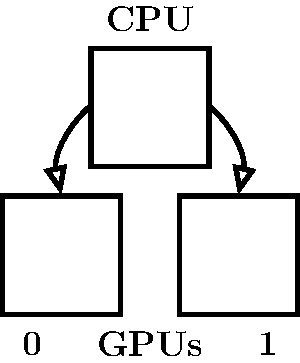
\includegraphics[width=\textwidth]{PaCT/copyDistribution_matrix}
    \caption{\emph{copy}}
    \label{fig:distributions_matrix:copy}
  \end{subfigure}
  \hfill
  \begin{subfigure}{.22\textwidth}
    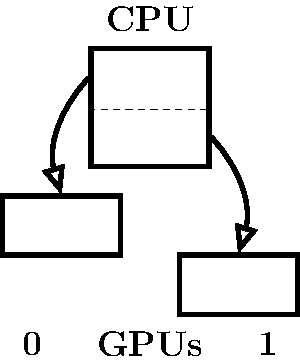
\includegraphics[width=\textwidth]{PaCT/blockDistribution_matrix}
    \caption{\emph{block}}
    \label{fig:distributions_matrix:block}
  \end{subfigure}
  \caption{Distributions of a matrix in SkelCL.}
  \label{fig:distributions_matrix}
\end{figure}


Three kinds of basic distributions are currently available in \SkelCL:
\emph{single}, \emph{copy}, and \emph{block} (see \autoref{fig:distributions} for distributing a vector on a system with two \GPUs).
If distribution is set to \emph{single} (\autoref{fig:distributions:single}), then vector's whole data is stored on a single \GPU (the first \GPU if not specified otherwise).
The \emph{copy} distribution (\autoref{fig:distributions:copy}) copies vector's entire data to each available \GPU.
With the \emph{block} distribution (\autoref{fig:distributions:block}), each \GPU stores a contiguous, disjoint chunk of the vector.

The same three distributions are provided also for the matrix data type as shown in \autoref{fig:distributions_matrix}.
The \emph{block} distribution (\autoref{fig:distributions_matrix:block}) splits the matrix into chunks of rows, which simplifies the implementation.

% In particular the overlap distribution splits the matrix into one chunk for each GPU; in addition, each chunk contains a number of continuous rows from the neighboring chunks.
% A parameter -- the \emph{overlap size} -- specifies the number of rows at the borders of a chunk which are copied to the two neighboring GPUs.
% \autoref{fig:Distribution_matrix:overlap} illustrates the overlap distribution:
% GPU 0 receives the top chunk ranging from the top row to the middle, while GPU 1 receives the second chunk ranging from the middle row to the bottom.
% The marked parts are called \emph{overlap region} they are the same on both GPUs.

The application developer can set the distribution of containers explicitly, otherwise every skeleton selects a default distribution for its input and output containers.
Container's distribution can be changed at runtime:
this implies data exchanges between multiple \GPUs and the \CPU, which are performed by the \SkelCL implementation implicitly.
As seen earlier in this chapter (\autoref{lst:lmosem:redistribution}) implementing such data transfers in the standard \OpenCL is a cumbersome task:
data has to be downloaded to the \CPU before it is uploaded to the \GPUs, including the corresponding length and offset calculations;
this results in a lot of low-level code which becomes completely hidden when using \SkelCL.

A special situation arises when the distribution is changed from the \emph{copy} distribution to any other distribution.
In this case each \GPU holds its own full copy of the data which might have been modified locally on each \GPU.
In order to maintain \SkelCL's concept of a self-contained container, these different versions are combined using a user-specified function when the distribution is changed.
If no function is specified, the copy of the first \GPU is taken as the new version of the container; the copies of the other \GPUs are discarded.


% ============================================================================ %
\subsection{More Complex Algorithmic Skeletons}
\label{section:skelcl-programming-model:specialSkeletons}

The basic algorithmic skeletons presented in~\autoref{section:skelcl-programming-model:skeletons} are long known in the functional and algorithmic skeleton communities.
In this section we will introduce two new more advanced algorithmic skeletons, which are more restrictive.
By limiting the use cases of these novel algorithmic skeleton we are able to make more assumptions in the implementation and provide advanced optimizations on modern multi-\GPU systems.

The first new skeleton (\stencil) is targeted towards \emph{stencil} (\aka nearest neighbor) computations, which are computations performed for every element of a container while including neighboring elements in the computation.
The second new skeleton (\allpairs) combines two matrix containers in an all-to-all fashion, which is a pattern used in applications like n-body simulation or matrix matrix multiplication.

For both skeletons we will first formally define them before looking at possible use cases.
Their implementations targeting multi-\GPU systems will be described in~\autoref{section:skelcl-library}.


\subsubsection{The \stencil Skeleton}

Many numerical and image processing applications dealing with two-dimensional data perform calculations for a particular data element taking neighboring data elements into account.
These type of applications are also known as \emph{stencil} or \emph{nearest neighbor} applications.
To facilitate the development of such applications, we introduce the \stencil skeleton that can be used with both vector and matrix data type.

The \stencil skeleton is customized with three parameters: a unary function $f$, an integer value $d$, and an out-of-bounds function $h$.
The skeleton applies $f$ to each element of an input container while taking the neighboring elements within the range $d$ in each dimension into account.
When neighboring elements are accesses at the boundaries of the container out of bound accesses occur.
In these cases the function $h$ is called with the index causing the out of bound access and should return a replacement value.
We now formally define the \stencil skeleton. We start with the definition for vectors:
\begin{definition}
  \label{definition:mapoverlap}
  Let $\vec{x}$ be a vector of size $n$ with elements $x_i$ where $0 < i \leq n$.
  Let $f$ be a customizing function, $d$ be a positive integer value, and $h$ be an out-of-bound handling function.
  The algorithmic skeleton \stencil is defined as follows:
  \begin{equation*}
    \begin{split}
    &stencil \big(\ f,\  d,\ h,\ [x_1, x_2, \dots, x_n]\ \big) \eqdef [y_1, y_2, \dots, y_n]\\
    &\text{where}\\[.5em]
    &\qquad y_i = f(x_{i-d}, \ldots, x_{i+d}) \ \ \forall\ i :  0 < i \leq n\\
    &\text{and\hfill}\\
    &\qquad x_j = h(j) \ \ \forall\ j : -d < j \leq 0\ \vee n < j \leq n+d
    \end{split}
  \end{equation*}
\end{definition}

\noindent
The definition for matrices is similar:
\begin{definition}
  \label{definition:mapoverlap:matrix}
  Let $M$ be an $n\times m$ matrix with elements $M_{i,j}$ where $0 < i \leq n$ and $0 < j \leq m$.
  Let $f$ be a customizing function, $d$ be an positive integer value, and $h$ be a out of bound handling function.
  The algorithmic skeleton \stencil is defined as follows:
  \begin{equation*}
    \begin{split}
    & stencil \big(\ f,\  d,\ h,\ \DottedMatrix{M_{0,0}}{M_{0,m}}{M_{n,0}}{M_{n,m}}\big)
               \eqdef \DottedMatrix{N_{0,0}}{N_{0,m}}{N_{n,0}}{N_{n,m}}\\
               &\text{where}\\[.5em]
    &\qquad N[i,j] = f\left(\DottedMatrix{M_{i-d,j-d}}{M_{i-d,j+d}}{M_{i+d,j-d}}{M_{i+d,j+d}}\right)\ \ \forall\ i,j
        \begin{array}{r} 0 < i \leq n,\\ 0 < j \leq m \end{array}\\
        &\text{and}\\
    &\qquad M[i,j] = h(i,j) \qquad \forall\ i,j \begin{array}{r} -d < j \leq 0\ \vee n < j \leq n+d,\\ -d < j \leq 0\ \vee m < j \leq m+d \end{array}
    \end{split}
  \end{equation*}
\end{definition}


SkelCL currently supports a fixed set of choices for the out-of-bound handling function $h$ motivated by common cases of of bound handling in image processing applications.
This restriction could easily be lifted in the future.
The \stencil skeleton can currently be configured to handle out of bound accesses in two possible ways:
\begin{enumerate}
  \item a specified neutral value is returned (\ie, the out of bound function $h$ is constant);
  \item the nearest valid value inside the container is returned.
\end{enumerate}

Possible applications for the stencil skeleton are image processing applications or physics simulations (see~\autoref{sec:imageProcessing} and \autoref{sec:physicsSim}).
A simple example application is the \emph{discrete Laplacian operator} used in image processing, \eg, for edge detection~\cite{Umbaugh1997}.
It computes a new value for every pixel of an image by weighting and summing up its direct neighboring pixel values, as follows:
\begin{align*}
  laplacian&(M) = stencil(\ f,\ 1,\ \overline{0},\ M\ )\\
  \text{where:} \ \ &
  \begin{array}{ll}%
  f &\left(\left[\begin{array}{lll}%
      \hspace{-.5em} M_{i-1,j-1}& \hspace{-.5em} M_{i-1,j} & \hspace{-.5em}M_{i-1,j+1}\vspace{-.25em}\\%
      \hspace{-.5em} M_{i,j-1}& \hspace{-.5em} M_{i,j} & \hspace{-.5em}M_{i,j+1}\vspace{-.25em}\\%
      \hspace{-.5em} M_{i+1,j-1}& \hspace{-.5em} M_{i+1,j} & \hspace{-.5em}M_{i+1,j+1}\vspace{-.25em}
    \end{array}\right] \right) = \\
          &\ M_{i-1,j} + M_{i,j-1} - 4 \times M_{i,j} + M_{i,j+1} + M_{i+1,j}
  \end{array} \\
  \text{and } \overline{0} \text{ is th}&\text{e constant function always returning 0.}
\end{align*}

\subsubsection{The overlap data distribution}

\begin{figure}[tb]
  \centering
  \begin{subfigure}[b]{.3\textwidth}
    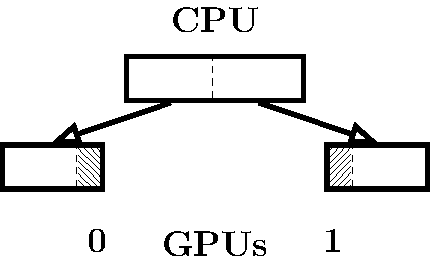
\includegraphics[width=\textwidth]{PaCT/overlapDistribution_vector}
    \caption{\emph{overlap}}
    \label{fig:overlap_distribution}
  \end{subfigure}
  \hspace{3em}
  \begin{subfigure}[b]{.22\textwidth}
    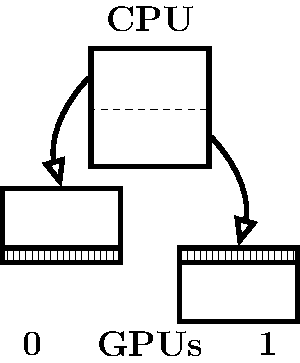
\includegraphics[width=\textwidth]{PaCT/overlapDistribution_matrix}
    \caption{\emph{overlap}}
    \label{fig:overlap_distribution:matrix}
  \end{subfigure}
  \caption{Overlap distribution of a vector and matrix in SkelCL.}
  \label{fig:overlap_distribution}
  \bigskip
\end{figure}

Together with the \stencil skeleton we introduce a new distribution called \emph{overlap} (Figure~\ref{fig:overlap_distribution}).
The overlap distribution splits the container into one chunk for each device, similarly to the \emph{block} distribution.
In addition, each chunk consists of a number of continuous elements (in case of the vector) or rows (in case of the matrix) which are copied to the neighboring devices, similar to the \emph{copy} distribution.
Therefore, the overlap distribution can be seen as a combination of the \emph{block} and \emph{copy} distribution.
The number of elements or rows at the edges of a chunk which are copied to the neighboring devices are called the \emph{overlap size}.

The \emph{overlap} distribution ensures that neighboring elements are always accessible even if the container is split across multiple devices.
The \emph{overlap} distribution is, therefore, automatically selected as distribution by the \stencil skeleton automatically setting the overlap size to the skeleton parameter $d$, which ensures that every device has access to the necessary neighboring elements.





\subsubsection{The \allpairs Skeleton}
\label{sec:allpairs_skeleton}

\emph{Allpairs computations} occur in a variety of applications, ranging from matrix multiplication and N-Body simulations in physics~\cite{AroraShVu2009} to pairwise Manhattan distance computations in bioinformatics~\cite{ChangDeQuRo2009}.
These applications share a common computational pattern:
for two sets of entities, the same computation is performed independently for all pairs in which entities from the first set are combined with entities from the second set.
We define the \allpairs skeleton to simplify the development of such applications.
We represent the entries of both sets as vectors of length $d$, where the cardinality of the first set is $n$ and the cardinality of the second set is $m$.
We model the first set as a $n\times d$ matrix $A$ and the second set as a $m\times d$ matrix $B$.
The allpairs computation yields an output matrix $C$ of size $n\times m$ with $c_{i, j} = A_i \oplus B_j$, where $A_i$ and $B_j$ are row vectors of $A$ and $B$, correspondingly,
%:
%$A_i = [A_{i,1}, \cdots, A_{i, d}]$, $B_j = [B_{j,1}, \cdots, B_{j,d}]$,
and $\oplus$ is a binary operator defined on vectors.

We formally define the \allpairs skeleton as follows:

\begin{definition}
  \label{def:allpairs}
  Let $A$ be a $n\times d$ matrix, $B$ be a $m\times d$ matrix, and $C$ be a $n\times m$ matrix, with their elements $A_{i,j}$, $B_{i,j}$, and $C_{i,j}$ respectively.
  The algorithmic skeleton \allpairs with customizing binary function $\oplus$ is defined as follows:
  \begin{equation*}
    \begin{split}
    allpairs&(\oplus)\left(%
      \left[ \begin{array}{ccc} A_{1,1} & \cdots & A_{1,d}\\[.25em] \vdots & & \vdots\\[.25em] A_{n,1} & \cdots & A_{n,d} \end{array}\right], %
      \left[ \begin{array}{ccc} B_{1,1} & \cdots & B_{1,d}\\[-.25em] \cdot & & \cdot\\[-.75em] \cdot & & \cdot\\[-.25em] B_{m,1} & \cdots & B_{m,d} \end{array}\right]%
      \right)\\
    &\eqdef \left[ \begin{array}{ccc} C_{1,1} & \cdots & C_{1,m}\\[.25em] \vdots & & \vdots\\[.25em] C_{n,1} & \cdots & C_{n,m} \end{array} \right]
    \end{split}
  \end{equation*}
  where elements $C_{i,j}$ of the $n\times m$ matrix $C$ are computed as follows:
  \[
    C_{i,j} = \DottedVector{A_{i,1}}{A_{i,d}} \oplus \DottedVector{B_{j,1}}{B_{j,d}}
  \]
\end{definition}

\autoref{fig:allpairs:access:not_transposed} illustrates this definition:
the element $C_{2,3}$ of matrix $C$ marked as \circled{3} is computed by combining the second row of $A$ marked as \circled{1} with the third row of $B$ marked as \circled{2} using the binary operator $\oplus$.
\autoref{fig:allpairs:access:transposed} shows the same computation with the transposed matrix $B$.
This visualization shows how the structure of matrix $C$ is determined by the two input matrices $A$ and $B$.

\begin{figure}[tb]
  \centering
  \begin{subfigure}[b]{.44\textwidth}
    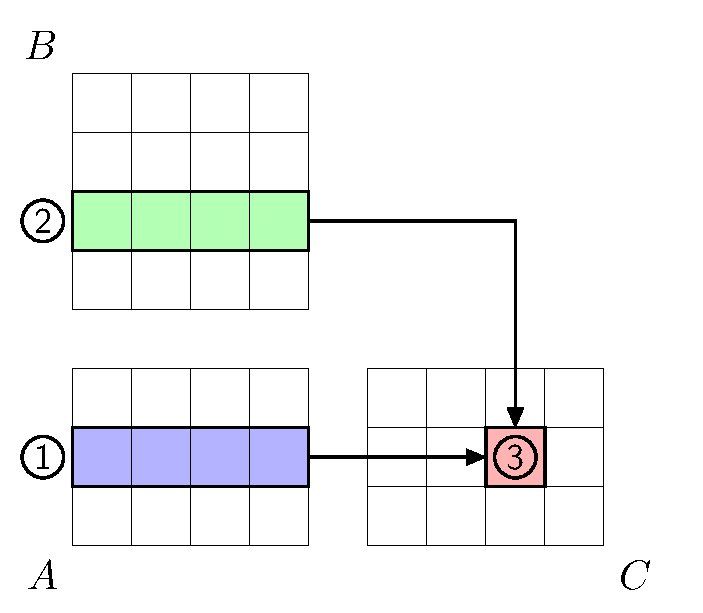
\includegraphics[width=\textwidth]{HLPP/allpairs_access_pattern_alternative}
    \caption{}
    \label{fig:allpairs:access:not_transposed}
  \end{subfigure}
  \hfill
  \begin{subfigure}[b]{.44\textwidth}
    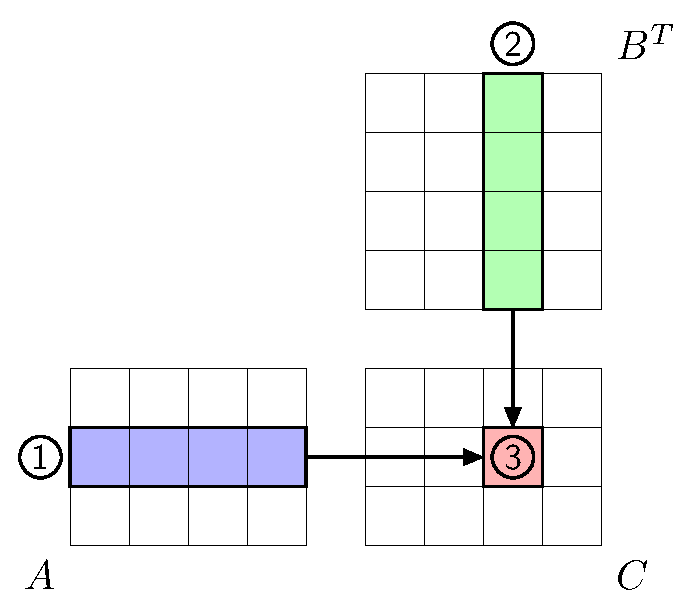
\includegraphics[width=\textwidth]{HLPP/allpairs_access_pattern}
    \caption{}
    \label{fig:allpairs:access:transposed}
  \end{subfigure}
  \caption{The allpairs computation schema. (\subref{fig:allpairs:access:not_transposed}): element $C_{2,3}$
    \protect\tikz[baseline=(char.base)]\protect\node[shape=circle,draw,inner sep=1pt] (char) {3};
    is computed by combining the second row of $A$
    \protect\tikz[baseline=(char.base)]\protect\node[shape=circle,draw,inner sep=1pt] (char) {1};
    with the third row of $B$
    \protect\tikz[baseline=(char.base)]\protect\node[shape=circle,draw,inner sep=1pt] (char) {2};
    using the binary operator $\oplus$. (\subref{fig:allpairs:access:transposed}): the same situation where the transpose of matrix $B$ is shown.}
  \label{fig:allpairs:access}
\end{figure}

Let us consider two example applications which can be expressed by customizing the \allpairs skeleton with a particular function $\oplus$.

\paragraph{Example 1:}
The Manhattan distance (or $L_1$ distance) is a measure of distance which is used in many applications.
In general, it is defined for two vectors, $x$ and $y$, of equal length $d$, as follows:
\begin{equation}
  \label{eq:man_dist}
  \ManDist(x, y) = \sum_{k=1}^d | x_k - y_k |
\end{equation}
In~\cite{ChangDeQuRo2009}, the so-called Pairwise Manhattan Distance (\emph{PMD}) is studied as a fundamental operation in hierarchical clustering for data analysis.
\emph{PMD} is obtained by computing the Manhattan distance for every pair of rows of a given matrix.
This computation for arbitrary matrix $A$ can be expressed using the \allpairs skeleton customized with the Manhattan distance defined in \autoref{eq:man_dist}:
\begin{equation}
  \PMD(A) = allpairs(\mbox{\emph{ManDist}})\left(A, A\right)
\end{equation}
The $n\times n$ matrix computed by the customized skeleton contains the Manhattan distance for every pair of rows of the input $n\times d$ matrix $A$.

\paragraph{Example 2:}
Matrix-matrix multiplication is a basic linear algebra operation, which is a building block of many scientific applications.
A $n\times d$ matrix $A$ is multiplied with a $d\times m$ matrix $B$, producing a $n\times m$ matrix $C=A\times B$ whose element $C_{i,j}$ is computed as the dot product of the $i$th row of $A$ with the $j$th column of $B$.
The dot product of two vectors, $a$ and $b$ of length $d$, is computed as follows:
\begin{equation}
  \dotProduct (a,b) = \sum_{k=1}^d a_k \cdot b_k
\end{equation}
The matrix multiplication can be expressed using the \allpairs skeleton as:
\begin{equation}
  A\times B = allpairs(\dotProduct)\left(A, B^T\right)
  \label{eq:mat_mult_allpairs}
\end{equation}
where $B^T$ is the transpose of matrix $B$.

% TODO: moved to impl ...
% \paragraph{The \allpairs skeleton using multiple GPUs}
% \label{sec:allpairs:multi_gpu}
% \begin{figure}[b]
%   \centering
%   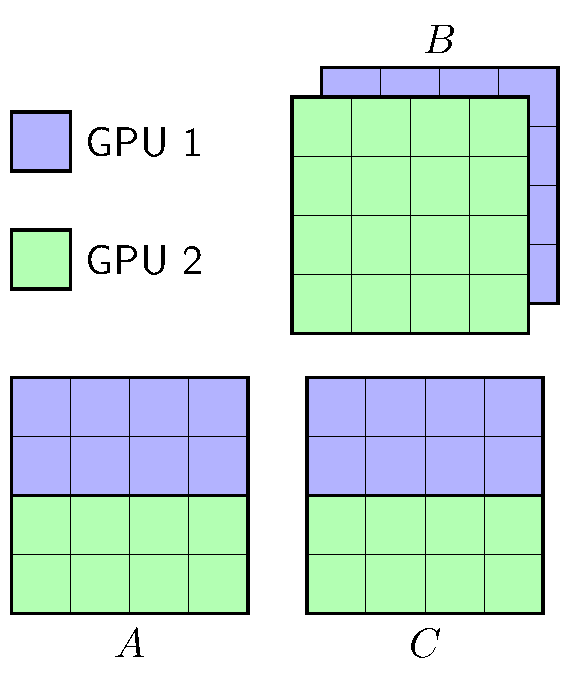
\includegraphics[width=.3\textwidth]{HLPP/multi_gpu}
%   \caption{Data distributions used for a system with two GPUs: matrices $A$ and $C$ are \emph{block} distributed, matrix $B$ is \emph{copy} distributed.}
%   \label{fig:multi_gpu}
% \end{figure}
% 
% The \allpairs skeleton can be efficiently implemented not only on systems with a single \GPU, but on multi-\GPU systems as well.
% The necessary data distribution can be easily expressed using two of \SkelCL's \emph{distributions}, as shown in \autoref{fig:multi_gpu}:
% Matrix $B$ is \emph{copy} distributed, \ie, it is copied entirely to all \GPUs in the system.
% Matrix $A$ and $C$ are \emph{block} distributed, \ie, they are row-divided into as many equally-sized blocks as \GPUs are available;
% each block is copied to its corresponding \GPU.
% Following these distributions, each \GPU computes one block of the result matrix $C$.
% In the example with two GPUs shown in \autoref{fig:multi_gpu}, the first two rows of $C$ are computed by \GPU 1 and the last two rows by \GPU 2.
% The \allpairs skeleton automatically selects these distributions, therefore, the same source code can be used when using a single \GPU or multiple \GPUs.



\subsubsection{The specialized \allpairs skeleton}
\label{sec:opt_allpairs_skeleton}
When targeting \GPU architectures, implementing an optimized version of the \allpairs skeleton is possible if certain assumptions about the customizing function $f$ can be made.
In this section, we will start by discussing the properties of $f$ necessary for an optimized \GPU implementation.
In particular we will analyze the memory access pattern of the matrix multiplication as the memory accesses turns out to be crucial for the performance.
We then observe that the identified memory access pattern can also be found in other allpairs computations and, therefore, define a specialized version of the allpairs skeleton, which is suitable for applications having this pattern.
% Finally, we estimate the gained efficiency by the optimized implementation over the generic one.


\paragraph{The memory access pattern of the matrix multiplication}
\begin{figure}[t]
  \centering
  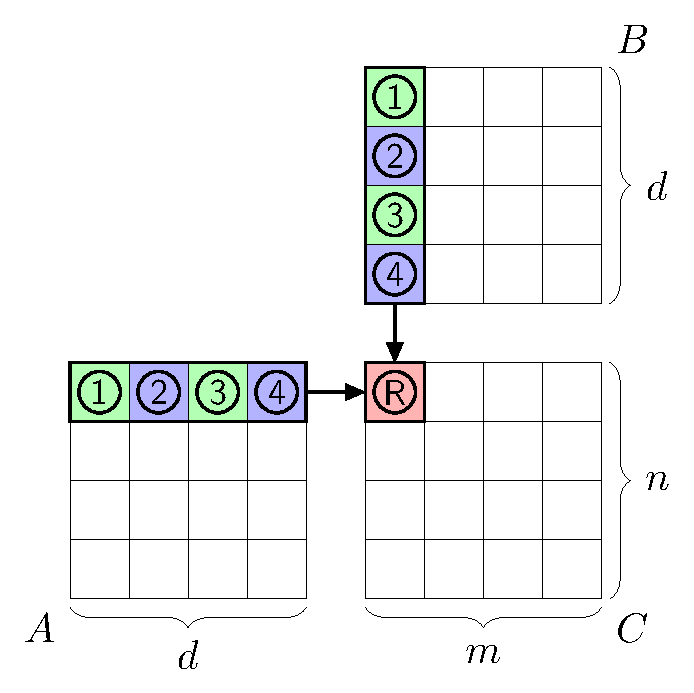
\includegraphics[width=0.4\textwidth]{HLPP/single_memory_access}
  \caption{The memory access pattern of the matrix multiplication $A\times B = C$.}
  \label{fig:mm_access_pattern}
\end{figure}
Figure~\ref{fig:mm_access_pattern} shows the memory access pattern of the matrix multiplication for $4\times 4$ matrices.
To compute the element \circled{R} of the result matrix $C$, the first row of matrix $A$ and the first column of matrix $B$ are combined.
In the skeleton-based code, these two vectors are used by the customizing function $f$, which is the dot product in case of the matrix multiplication.
The dot product performs a pairwise multiplication of the two vectors and then sums up the intermediate result.
In the example, the two elements marked as \circled{1} are multiplied first and the intermediate result is stored;
then, the next elements (marked as \circled{2}) are multiplied and the result is added to the intermediate result, and so forth.
% TODO: Moved to impl section ...
% Let us assume targeting \GPU architectures and estimate the number of global (and therefore expensive) memory accesses required for computing an element of the matrix multiplication in the generic case.
% One global memory read access for every element of both input vectors is performed, and a single global memory write access is required to write the result into the output matrix.
% Therefore, 
% \begin{equation}
%   n\cdot m\cdot (d + d + 1)
%   \label{eq:mm:accesses}
% \end{equation}
% global memory accesses are performed in total, where $n$ and $m$ are the height and width of matrix $C$ and $d$ is the width of $A$ and the height of $B$.
% By using the fast but small local memory this number of global memory accesses can be reduces and, thus, performance can be improved.
% Using the local memory for matrix matrix multiplication is a well known optimization.

A key observation is, that other applications share the same memory access pattern as the matrix multiplication shown in \autoref{fig:mm_access_pattern}.
For example, the customizing function of the pairwise Manhattan distance as defined by \autoref{eq:man_dist} follows obviously the same memory access pattern as the matrix multiplication.
To find a common representation for a customizing function with this pairwise access pattern, we describe it as a sequential composition of two basic algorithmic skeletons: \zip and \reduce.
The \emph{sequential composition} composition of two functions (or skeletons) $f$ and $g$ is denoted by $g \circ f$ which means that $f$ is applied first and then $g$ is applied to the result value of $f$ as input, \ie, $(g\circ f)(x) = g(f(x))$.

For the \reduce skeleton customized with $\oplus$ and corresponding identity element $id$, and the \zip skeleton customized with $\otimes$ we can sequentially compose them as follows:
\begin{eqnarray*}
  reduce\ (\oplus, id) \circ zip\big(\ \otimes,\ a,\ b\ \big) &=&\\
  reduce\ (\oplus, id) \big(\ zip\big(\ \otimes,\ \DottedVector{a_1}{a_n},\ \DottedVector{b_1}{b_n}\ \big)\ \big) &=&\\
  (a_1 \otimes b_1)\ \ \oplus &\cdots& \oplus\ \ (a_n \otimes b_n)
\end{eqnarray*}

This composition of the two customized skeletons yields a function which we denote \zipReduce; it takes two input vectors and produces a single scalar value:

\begin{equation*}
  zipReduce\big(\oplus,\ id,\ \otimes,\ a,\ b\ \big) \eqdef 
  reduce\ (\oplus,\ id) \circ zip\big(\ \otimes,\ a,\ b\ \big)
\end{equation*}

Following the definition of \zipReduce, we can express the customizing function of the Manhattan distance as follows.
We use the binary operator $a \ominus b = |a - b|$ as the customizing function for \zip, and addition as the customizing function for the \reduce skeleton:
\begin{eqnarray*}
    \ManDist(a, b) &=& \sum_{i=1}^{n} | a_i - b_i | = (a_1 \ominus b_1) + \cdots + (a_n \ominus b_n)\\
    &=& zipReduce\big(+,\ 0,\ \ominus,\ \DottedVector{a_1}{a_n},\ \DottedVector{b_1}{b_n}\big)
\end{eqnarray*}

Similarly, we can express the dot product (which is the customizing function of matrix multiplication) as a \zip-\reduce composition, by using multiplication for customizing the \zip skeleton and addition for customizing the \reduce skeleton:
\begin{eqnarray*}
  \dotProduct(a, b) &=& \sum_{i = 1}^{n} a_i \cdot b_i = (a_1 \cdot b_1) + \cdots + (a_n \cdot b_n)\\
  &=& zipReduce\big(+,\ 0,\ \times,\ a,\ b\big)
\end{eqnarray*}

\paragraph{Definition of the specialized \allpairs skeleton}

We can now specialize the generic Definition~\autoref{def:allpairs} of the \allpairs skeleton by employing the sequential composition of the customized \reduce and \zip skeletons for customizing the \allpairs skeleton.
From here on, we refer to this specialization as the \allpairs skeleton \emph{customized with \zip-\reduce}.

\begin{definition}
  \label{def:allpairs:specialized}
  Let $A$ be a $n\times d$ matrix, $B$ be a $m\times d$ matrix, and $C$ be a $n\times m$ matrix, with their elements $A_{i,j}$, $B_{i,j}$, and $C_{i,j}$ respectively.
  Let $\oplus$ be an associative and commutative, binary customizing operator with the corresponding identity element $id$.
  Let $\otimes$ be a binary customizing operator.
  The specialized algorithmic skeleton \allpairs customized with \zip-\reduce is defined as follows:
  \begin{equation*}
    \begin{split}
    allpairs&(\oplus,\ id,\ \otimes)\left(%
      \left[ \begin{array}{c} A_{1,1} \cdots A_{1,d}\\[.25em] \vdots \hspace{4em} \vdots\\[.25em] A_{n,1} \cdots A_{n,d} \end{array}\right], %
      \left[ \begin{array}{c} B_{1,1} \cdots B_{1,d}\\[-.25em] \cdot \hspace{4em} \cdot\\[-.75em] \cdot \hspace{4em} \cdot\\[-.25em] B_{m,1} \cdots B_{m,d} \end{array}\right]%
      \right)\\
    &\eqdef \left[ \begin{array}{ccc} C_{1,1} & \cdots & C_{1,m}\\[.25em] \vdots & & \vdots\\[.25em] C_{n,1} & \cdots & C_{n,m} \end{array} \right]
    \end{split}
  \end{equation*}
  where elements $C_{i,j}$ of the $n\times m$ matrix $C$ are computed as follows:
  \[
    C_{i,j} = zipReduce(\oplus, id, \otimes, \DottedVector{A_{i,1}}{A_{i,d}}, \DottedVector{B_{j,1}}{B_{j,d}})
  \]
\end{definition}


While not every allpairs computation can be expressed using this specialization, many real-world problems can.
In addition to the matrix multiplication and the pairwise Manhattan distance examples are the pairwise computation of the Pearson correlation coefficient~\cite{ChangDeQuRo2009} and estimation of Mutual Informations~\cite{DaubStSeKl2004}.
The composition of \zip and \reduce is well known in the functional programming world.
Google's popular \emph{MapReduce} programming model has been inspired by a similar composition of the \map and \reduce skeletons.
\cite{Laemmel2007} extensively discusses the relation of MapReduce to functional programming.


% TODO: Moved to impl ...
% \paragraph{Estimation of the performance gain of specialization}
% By expressing the customizing function of the \allpairs skeleton as a \zip-\reduce composition, we provide additional semantic information about the memory access pattern of the customizing function to the skeleton implementation, thus allowing for improving the performance.
% Our idea of optimization is based on the OpenCL programming model that organizes \emph{work-items} (i.\,e., threads executing a kernel) in \emph{work-groups} which share the same \GPU local memory.
% By loading data needed by multiple work-items of the same work-group into the local memory, we can avoid repetitive accesses to the global memory.
% 
% \begin{figure}[b]
%   \centering
%   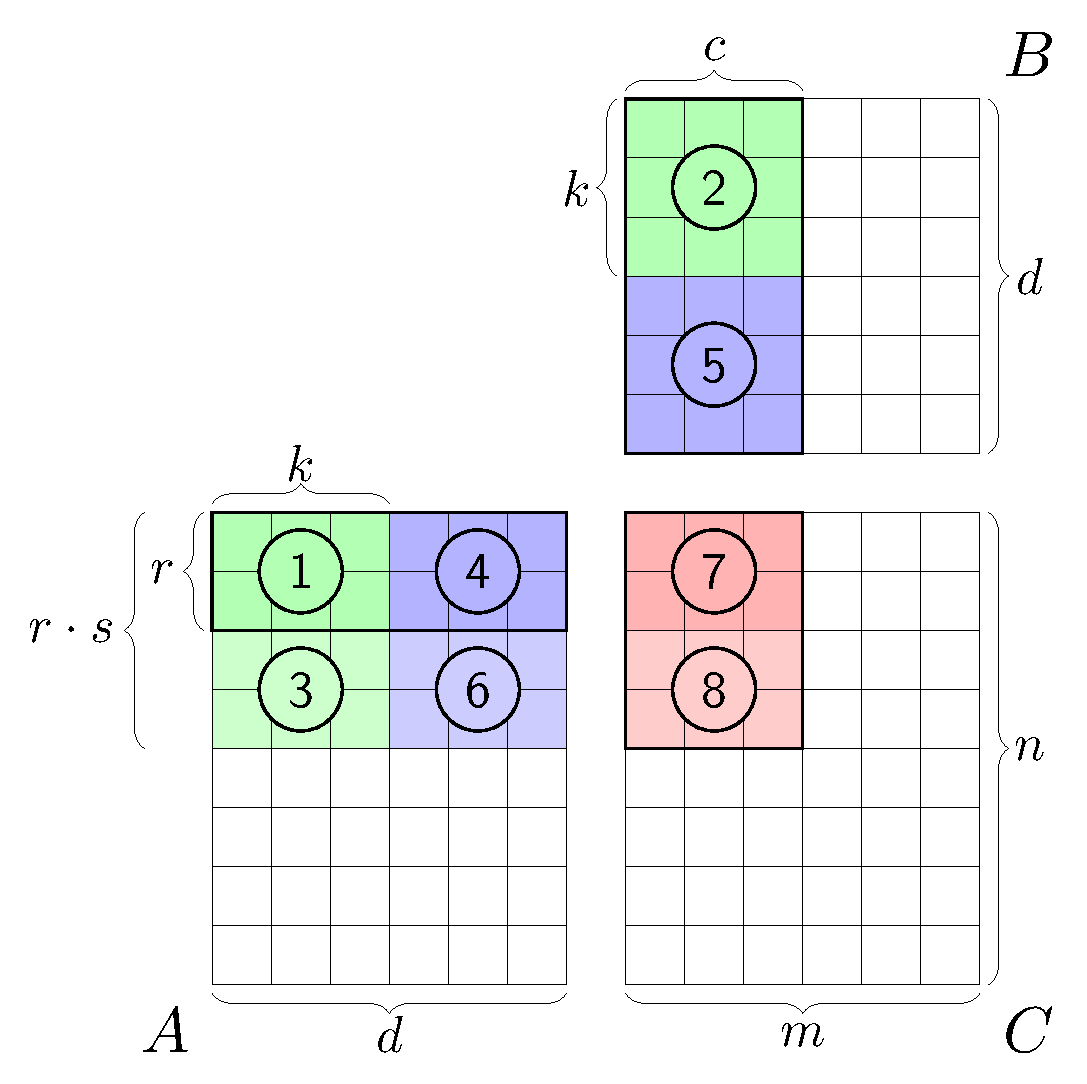
\includegraphics[width=.4\textwidth]{HLPP/memory_access}
%   \caption{Implementation schema of the specialized allpairs skeleton.}
%   \label{fig:memory_access}
% \end{figure}
% For the \allpairs skeleton with the \zip-\reduce customizing function, we can adopt the implementation schema for \GPUs~\cite{SarjeAl2013}, as shown in Figure~\ref{fig:memory_access}.
% We allocate two arrays in the local memory, one of size $r\times k$ ($r=2$, $k=3$ in Figure~\ref{fig:memory_access}) for elements of $A$ and one of size $k\times c$ ($c=3$ in Figure~\ref{fig:memory_access}) for elements of $B$.
% A work-group consisting of $c\times r$ work-items computes $s$ blocks ($s=2$ in Figure~\ref{fig:memory_access}) of the result matrix $C$.
% In Figure~\ref{fig:memory_access}, the two blocks marked as \circled{7} and \circled{8} are computed by the same work-group as follows.
% In the first iteration, the elements of blocks \circled{1} and \circled{2} are loaded into the local memory and combined following the zip-reduce pattern.
% The obtained intermediate result is stored in block \circled{7}.
% Then, the elements of block \circled{3} are loaded and combined with the elements from \circled{2} which still reside in the local memory.
% The intermediate result is stored in block \circled{8}.
% In the second iteration, the algorithm continues in the same manner with blocks \circled{4}, \circled{5}, and \circled{6}, but this time, the elements of the blocks are also combined with the intermediate results of the first iteration, which are stored in blocks \circled{7} and \circled{8}.
% The advantage of computing multiple blocks by the same work-group is that we keep the elements of $B$ in the local memory when computing the intermediate results, \ie, we do not reload block \circled{2} twice for the computation of blocks \circled{7} and \circled{8}.
% 
% Every element loaded from the global memory is used by multiple work-items:
% \eg, the upper left element of block \circled{1} is loaded only once from the global memory, but used three times:
% in the computation of the upper left, upper middle, and upper right elements of \circled{7}.
% In general, every element loaded from $A$ is reused $c$ times, and every element from $B$ is reused $r\cdot s$ times.
% As the intermediate results are stored in the global memory of matrix $C$, we perform two additional memory accesses (read/write) for every iteration, \ie, $2\cdot \frac{d}{k}$ in total.
% Therefore, instead of $n\cdot m\cdot (d + d + 1)$ (see \autoref{eq:mm:accesses}) global memory accesses necessary when using the non-specialized skeleton and, thus, only the global memory, only
% \begin{equation}
%   n\cdot m\cdot (\frac{d}{r\cdot s} + \frac{d}{c} + 2\cdot \frac{d}{k})
% \end{equation}
% global memory accesses are performed.
% By increasing the parameters $s$ and $k$, or the number of work-items in a work-group ($c$ and $r$), more global memory accesses can be saved.
% However, the work-group size is limited by the \GPU hardware.
% While the parameters can be chosen independently of the matrix sizes, we have to consider the amount of available local memory.
% \cite{Friese2013}~and~\cite{SarjeAl2013}~discusses how suitable parameters can be found by performing runtime experiments.
% In~\cite{Friese2013} the parameters $c = 32$, $r=8$, $s=32$, and $k=64$ are used on modern \GPU hardware showing good performance.
% 
% We will report measurements of the performance difference for the two skeleton implementations on real hardware in \autoref{chapter:skelcl:apps}.
% 
% 

